\documentclass[12pt]{standalone}
\usepackage{circuitikz}

\usetikzlibrary{shapes.geometric}

%DEFINE COMPONENTS
\tikzset{register/.style={flipflop,
    flipflop def={t2=$\,$, t5=$\,$, cu=1},
    transform shape,
    scale=.5
}}

\tikzset{register enable/.style={flipflop,
    flipflop def={t2=$\,$, t5=$\,$, cu=1, td=EN},
    transform shape,
    scale=.5
}}

\tikzset{two io register/.style={flipflop,
    flipflop def={t1=$\,$, t3=$\,$, t4=$\,$, t6=$\,$, cu=1},
    transform shape,
    scale=.5
}}

\tikzset{two input mux/.style={muxdemux,
    muxdemux def={Lh=4, Rh=2, NL=2, NT=1, NB=0, NR=1},
    scale=.4
}}

\tikzset{four input mux/.style={muxdemux,
    muxdemux def={Lh=6, Rh=4, NL=4, NT=1, NB=0, NR=1},
    scale=.4
}}

\ctikzset{logic ports=ieee,
          multipoles/flipflop/clock wedge size=0.4,
          multipoles/external pins width=.5,
          multipoles/dipchip/width=2.5,
          multipoles/dipchip/pin spacing = 0.75}

\begin{document}

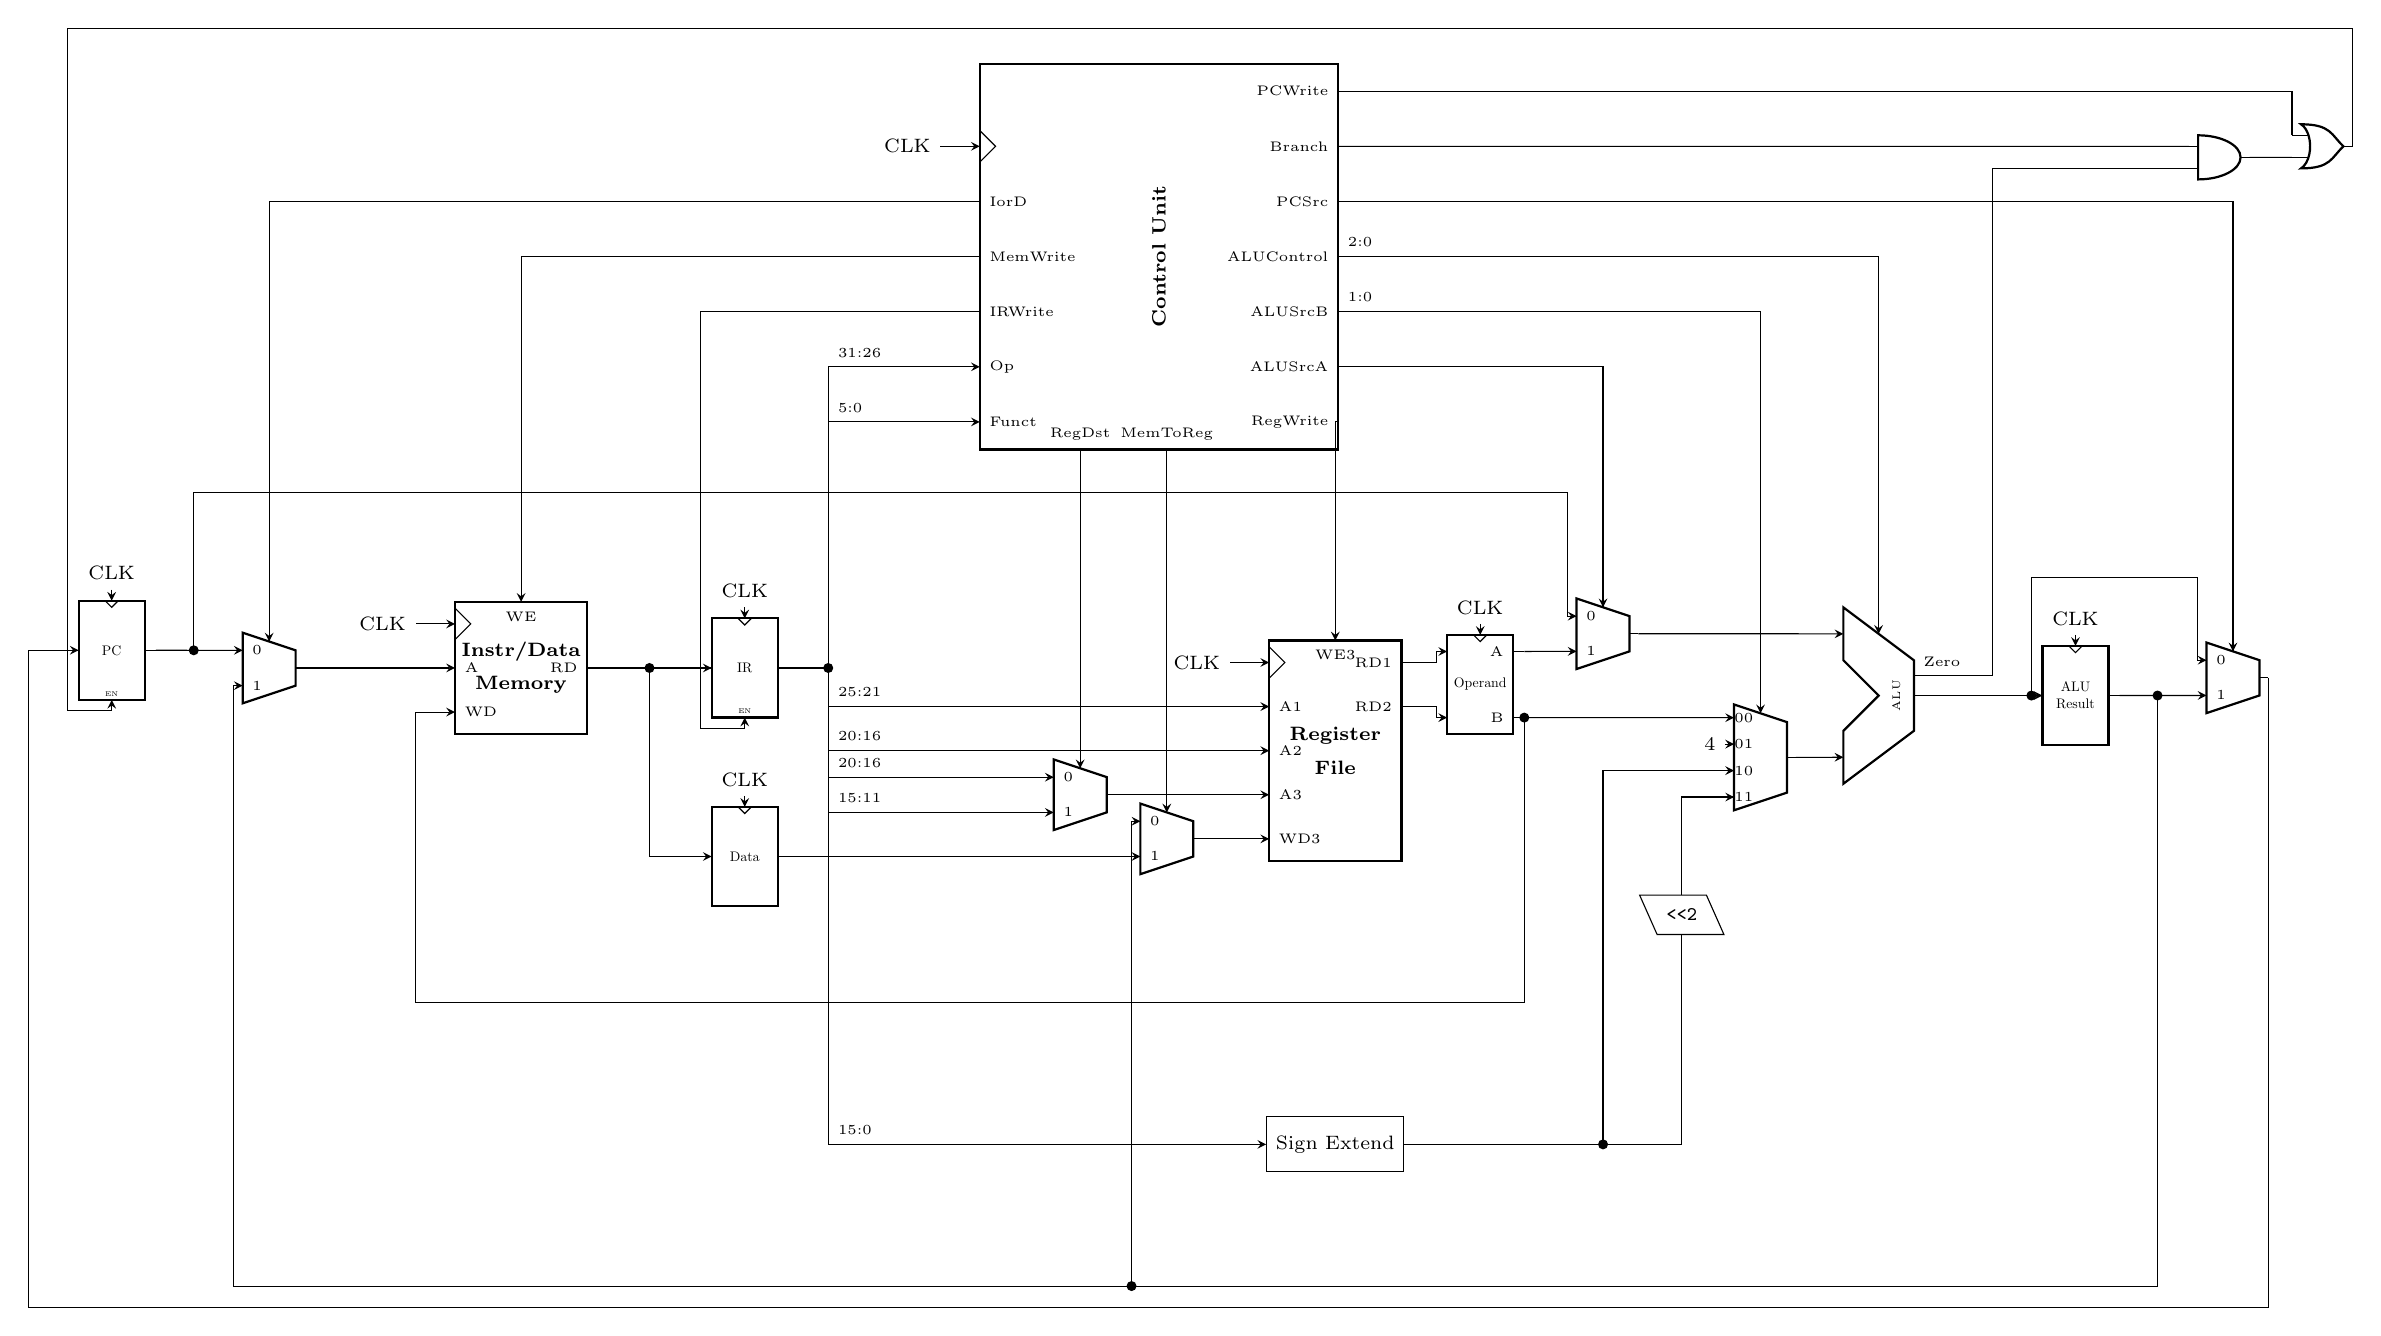
\begin{tikzpicture}
    
    %COMPONENTS---------------

    %Program Counter
    \node[register enable] (PC) at (0,0) {PC};
    \node[above, font=\scriptsize] at (PC.up) {CLK};
    \draw[-stealth] (PC.up) -- (PC.bup);
    
    %PC Mux
    \node[two input mux] (PC_mux) at ($ (PC) + (2,-.225) $) {};
    \node[right, font=\tiny] at (PC_mux.blpin 1) {0};
    \node[right, font=\tiny] at (PC_mux.blpin 2) {1};

    %Instr/Data Memory
    \node[dipchip, num pins=6, hide numbers, no topmark, align=center, external pins width=0] (memory) at ($ (PC_mux) + (3.2,0) $) {\scriptsize\textbf{Instr/Data} \\ \scriptsize\textbf{Memory}};
    \draw (memory.bpin 1) ++(0,0.2) -- ++(0.2,-0.2) -- ++(-0.2,-0.2);
    \draw[stealth-] (memory.bpin 1) -- ++(-.5,0) node[left, font=\scriptsize] {CLK};
    \node[right, font=\tiny] at (memory.bpin 2) {A};
    \node[right, font=\tiny] at (memory.bpin 3) {WD};
    \node[left, font=\tiny] at (memory.bpin 5) {RD};
    \node[below, font=\tiny] at (memory.n) {WE};

    %Instruction register
    \node[register enable] (IR) at ($ (memory.bpin 5) + (2,0) $) {IR};
    \node[above, font=\scriptsize] at (IR.up) {CLK};
    \draw[-stealth] (IR.up) -- (IR.bup);

    %Register File
    \node[dipchip, num pins=10, hide numbers, no topmark, align=center, external pins width=0] (regfile) at ($ (IR) + (7.5,-1.05) $) {\scriptsize\textbf{Register} \\ \scriptsize\textbf{File}};
    \draw (regfile.bpin 1) ++(0,0.2) -- ++(0.2,-0.2) -- ++(-0.2,-0.2);
    \draw[stealth-] (regfile.bpin 1) -- ++(-.5,0) node[left, font=\scriptsize] {CLK};
    \node[right, font=\tiny] at (regfile.bpin 2) {A1};
    \node[right, font=\tiny] at (regfile.bpin 3) {A2};
    \node[right, font=\tiny] at (regfile.bpin 4) {A3};
    \node[right, font=\tiny] at (regfile.bpin 5) {WD3};
    \node[left, font=\tiny] at (regfile.bpin 9) {RD2};
    \node[left, font=\tiny] at (regfile.bpin 10) {RD1};
    \node[below, font=\tiny] at (regfile.n) {WE3};

    %RegDst Mux
    \node[two input mux] (RegDst_mux) at ($ (regfile.bpin 4) - (2.4,0) $) {};
    \node[right, font=\tiny] at (RegDst_mux.blpin 1) {0};
    \node[right, font=\tiny] at (RegDst_mux.blpin 2) {1};
    
    %MemToReg Mux
    \node[two input mux] (MemToReg_mux) at ($ (regfile.bpin 5) - (1.3,0) $) {};
    \node[right, font=\tiny] at (MemToReg_mux.blpin 1) {0};
    \node[right, font=\tiny] at (MemToReg_mux.blpin 2) {1};
    
    %Data register
    \node[register] (Data) at (IR |- MemToReg_mux.blpin 2) {Data};
    \node[above, font=\scriptsize] at (Data.up) {CLK};
    \draw[-stealth] (Data.up) -- (Data.bup);

    %Operand register
    \node[two io register] (Operand) at ($ (regfile.bpin 9) !0.5! (regfile.bpin 10) + (1,0) $) {Operand};
    \node[left, font=\tiny] at (Operand.bpin 4) {B};
    \node[left, font=\tiny] at (Operand.bpin 6) {A};
    \node[above, font=\scriptsize] at (Operand.up) {CLK};
    \draw[-stealth] (Operand.up) -- (Operand.bup);

    %SrcA mux
    \node[two input mux] (SrcA_mux) at ($ (Operand.pin 6) + (1,.225) $) {};
    \node[right, font=\tiny] at (SrcA_mux.blpin 1) {0};
    \node[right, font=\tiny] at (SrcA_mux.blpin 2) {1};

    %SrcB mux
    \node[four input mux] (SrcB_mux) at ($ (Operand.pin 4) + (3,-.505) $) {};
    \node[right, font=\tiny] at ($ (SrcB_mux.blpin 1) - (.12,0) $) {00};
    \node[right, font=\tiny] at ($ (SrcB_mux.blpin 2) - (.12,0) $) {01};
    \node[right, font=\tiny] at ($ (SrcB_mux.blpin 3) - (.12,0) $) {10};
    \node[right, font=\tiny] at ($ (SrcB_mux.blpin 4) - (.12,0) $) {11};
    \draw[-stealth] (SrcB_mux.lpin 2) node[left, font=\scriptsize] {4} -- (SrcB_mux.blpin 2);

    %ALU
    \node[ALU, scale=.8, font=\tiny, external pins width=0] (ALU) at ($ (SrcA_mux) !0.5! (SrcB_mux) + (2.5,0) $) {\rotatebox{90}{ALU}};

    %ALU result register
    \node[register, align=center] (ALURes) at ($ (ALU) + (2.5,0) $) {ALU \\ Result};
    \node[above, font=\scriptsize] at (ALURes.up) {CLK};
    \draw[-stealth] (ALURes.up) -- (ALURes.bup);
    
    %ALU result mux
    \node[two input mux] (ALURes_mux) at ($ (ALURes) + (2,.225) $) {};
    \node[right, font=\tiny] at (ALURes_mux.blpin 1) {0};
    \node[right, font=\tiny] at (ALURes_mux.blpin 2) {1};

    %Sign extend
    \node[draw, rectangle, align=center, font=\scriptsize, minimum height=.7cm] (SE) at ($ (regfile) - (0,5) $) {Sign Extend};

    %<<2
    \node[trapezium,draw,trapezium left angle=120,trapezium right angle=60,trapezium stretches=true,minimum height=.5cm, font=\scriptsize\ttfamily] (ll2) at ($ (SrcB_mux) - (1,2) $) {<<2}; 

    %Control Unit
    \ctikzset{multipoles/dipchip/width=3.25}
    \node[dipchip, num pins=14, hide numbers, no topmark, align=center, external pins width=0, circuitikz/multipoles/dipchip/pin spacing = 0.5] (CU) at (13.3,5) {\rotatebox{90}{\scriptsize \textbf{Control Unit}}};
    \draw (CU.bpin 2) ++(0,0.2) -- ++(0.2,-0.2) -- ++(-0.2,-0.2);
    \draw[stealth-] (CU.bpin 2) -- ++(-.5,0) node[left, font=\scriptsize] {CLK};
    \node[right, font=\tiny] at (CU.bpin 3) {IorD};
    \node[right, font=\tiny] at (CU.bpin 4) {MemWrite};
    \node[right, font=\tiny] at (CU.bpin 5) {IRWrite};
    \node[right, font=\tiny] at (CU.bpin 6) {Op};
    \node[right, font=\tiny] at (CU.bpin 7) {Funct};
    \node[left, font=\tiny] at (CU.bpin 8) {RegWrite};
    \node[left, font=\tiny] at (CU.bpin 9) {ALUSrcA};
    \node[left, font=\tiny] at (CU.bpin 10) {ALUSrcB};
    \node[left, font=\tiny] at (CU.bpin 11) {ALUControl};
    \node[left, font=\tiny] at (CU.bpin 12) {PCSrc};
    \node[left, font=\tiny] at (CU.bpin 13) {Branch};
    \node[left, font=\tiny] at (CU.bpin 14) {PCWrite};

    %AND/OR gates
    \node[and port, scale=.5] (and) at ($ (CU.bpin 13) + (11.5,-.14) $) {};
    \node[or port, scale=.5] (or) at ($ (and.in 1) + (2,0) $) {};

    %LINKS---------------------

    %PC -> (...)
    \draw[-stealth] (PC.pin 5) -- (PC_mux.blpin 1);
    \draw[-stealth] ($ (PC.bpin 5) !0.5! (PC_mux.blpin 1) $) node[circ] {} -- ++(0,2) -| (SrcA_mux.lpin 1) -- (SrcA_mux.blpin 1);

    %PC_mux -> (...)
    \draw[-stealth] (PC_mux.rpin 1) -- (memory.pin 2);

    %Memory -> (...)
    \draw[-stealth] (memory.pin 5) -- (IR.bpin 2);
    \draw[-stealth] ($ (memory.pin 5) !0.5! (IR.bpin 2) $) node[circ] {} |- (Data.bpin 2);

    %IR -> (...) (top-down)
    \draw[-stealth] (IR.pin 5) -- ++(.5,0) node[circ] (IR_int) {} 
                    -- (IR_int |- CU.pin 6) node[above right, font=\tiny] {31:26}
                    -- (CU.pin 6);
    \draw[-stealth] (IR_int |- CU.pin 7) node[above right, font=\tiny] {5:0} -- (CU.pin 7);
    \draw[-stealth] (IR_int |- regfile.pin 2) node[above right, font=\tiny] {25:21} -- (regfile.pin 2);
    \draw[-stealth] (IR_int |- regfile.pin 3) node[above right, font=\tiny] {20:16} -- (regfile.pin 3);
    \draw[-stealth] (IR_int |- RegDst_mux.blpin 1) node[above right, font=\tiny] {20:16} -- (RegDst_mux.blpin 1);
    \draw[-stealth] (IR_int |- RegDst_mux.blpin 2) node[above right, font=\tiny] {15:11} -- (RegDst_mux.blpin 2);
    \draw[-stealth] (IR_int) -- (IR_int |- SE.west) node[above right, font=\tiny] {15:0}
                    -- (SE.west);

    %Data -> (...)
    \draw[-stealth] (Data.pin 5) -- (MemToReg_mux.blpin 2);

    %RegDst_mux -> (...)
    \draw[-stealth] (RegDst_mux.rpin 1) -- (regfile.pin 4);

    %MemToReg_mux -> (...)
    \draw[-stealth] (MemToReg_mux.rpin 1) -- (regfile.pin 5);

    %RegFile -> (...)
    \draw[-stealth] (regfile.pin 9) -| (Operand.pin 3) -- (Operand.bpin 3);
    \draw[-stealth] (regfile.pin 10) -| (Operand.pin 1) -- (Operand.bpin 1);

    %Operand -> (...)
    \draw[-stealth] (Operand.pin 6) -- (SrcA_mux.blpin 2);
    \draw[-stealth] (Operand.pin 4) -- (SrcB_mux.blpin 1);
    \draw[-stealth] (Operand.pin 4) node [circ] {}
                    |- ($ (regfile.south) !0.5! (SE) $) 
                    -| ($ (memory.bpin 3) - (.5,0) $) -- (memory.bpin 3);

    %SrcA_mux -> (...)
    \draw[-stealth] (SrcA_mux.rpin 1) -- (ALU.blpin 1);

    %SrcB_mux -> (...)
    \draw[-stealth] (SrcB_mux.rpin 1) -- (ALU.blpin 2);

    %ALU -> (...)
    \draw[-stealth] (ALU.rpin 1) -- (ALURes.bpin 2);
    \draw[-stealth] (ALURes.pin 2) node[circ] {}
                    -- ++(0,1.5) -| (ALURes_mux.lpin 1) -- (ALURes_mux.blpin 1);
    \draw ($ (ALU.rpin 1) + (0,.25) $) node[above right, font=\tiny] {Zero}
                    -- ++(1,0) |- (and.in 2);

    %ALURes -> (...)
    \draw[-stealth] (ALURes.pin 5) -- (ALURes_mux.blpin 2);
    \draw[-stealth] ($ (ALURes.bpin 5) !0.5! (ALURes_mux.blpin 2) $) node[circ] {}
                    -- ++(0,-7.5) coordinate (ALURes_int)
                    -| (PC_mux.lpin 2) -- (PC_mux.blpin 2);
    \draw[-stealth] (ALURes_int -| MemToReg_mux.lpin 1) node[circ] {}
                    -- (MemToReg_mux.lpin 1) -- (MemToReg_mux.blpin 1);

    %ALURes_mux -> (...)
    \draw[-stealth] (ALURes_mux.rpin 1) -- ++(0,-8) -| ($ (PC.pin 2) - (.5,0) $) -- (PC.bpin 2); 

    %SignExtend,<<2 -> (...)
    \draw[-stealth] (SE.east) -| (ll2.south) (ll2.north) |- (SrcB_mux.blpin 4);
    \draw[-stealth] ($ (SE -| ll2) - (1,0) $) node[circ] {} |- (SrcB_mux.blpin 3);

    %ControlUnit -> (...)
    \draw[-stealth] (CU.pin 3) -| (PC_mux.btpin 1);
    \draw[-stealth] (CU.pin 4) -| (memory.north);
    \draw[-stealth] (CU.pin 5) -| (IR.pin 2) |- (IR.down) -- (IR.bdown);
    \draw[-stealth] (CU.south -| RegDst_mux.tpin 1) node [above, font=\tiny] {RegDst} -- (RegDst_mux.btpin 1);
    \draw[-stealth] (CU.south -| MemToReg_mux.tpin 1) node [above, font=\tiny] {MemToReg} -- (MemToReg_mux.btpin 1);
    \draw[-stealth] (CU.pin 8) -| (regfile.north);
    \draw[-stealth] (CU.pin 9) -| (SrcA_mux.btpin 1);
    \draw[-stealth] (CU.pin 10) node[above right, font=\tiny] {1:0}  -| (SrcB_mux.btpin 1);
    \draw[-stealth] (CU.pin 11) node[above right, font=\tiny] {2:0} -| (ALU.btpin 1);
    \draw[-stealth] (CU.pin 12) -| (ALURes_mux.btpin 1);
    \draw (CU.pin 13) -- (and.in 1);
    \draw (CU.pin 14) -| (or.in 1);

    %AND/OR Gates
    \draw (and.out) -- (or.in 2);
    \draw[-stealth] (or.out) -- ++(0,1.5) -| (PC.pin 2) |- (PC.down) -- (PC.bdown);

\end{tikzpicture}

\end{document}